\documentclass[tikz,border=2mm]{standalone}
\usetikzlibrary{shapes.geometric, arrows}

\tikzstyle{startstop} = [ellipse, minimum width=2cm, minimum height=1cm,text centered, draw=black, fill=gray!20]
\tikzstyle{process} = [rectangle, minimum width=3cm, minimum height=1cm, text centered, draw=black, fill=blue!20]
\tikzstyle{decision} = [diamond, minimum width=3cm, minimum height=1cm, text centered, draw=black, fill=green!20, aspect=2]
\tikzstyle{bola} = [circle, minimum width=1cm, minimum height=1cm, text centered, draw=black, aspect=2]
\tikzstyle{delay} = [regular polygon, regular polygon sides=6, minimum width=2.5cm, minimum height=1cm, text centered, draw=black, fill=orange!20]
\tikzstyle{arrow} = [thick,->,>=stealth]

\begin{document}
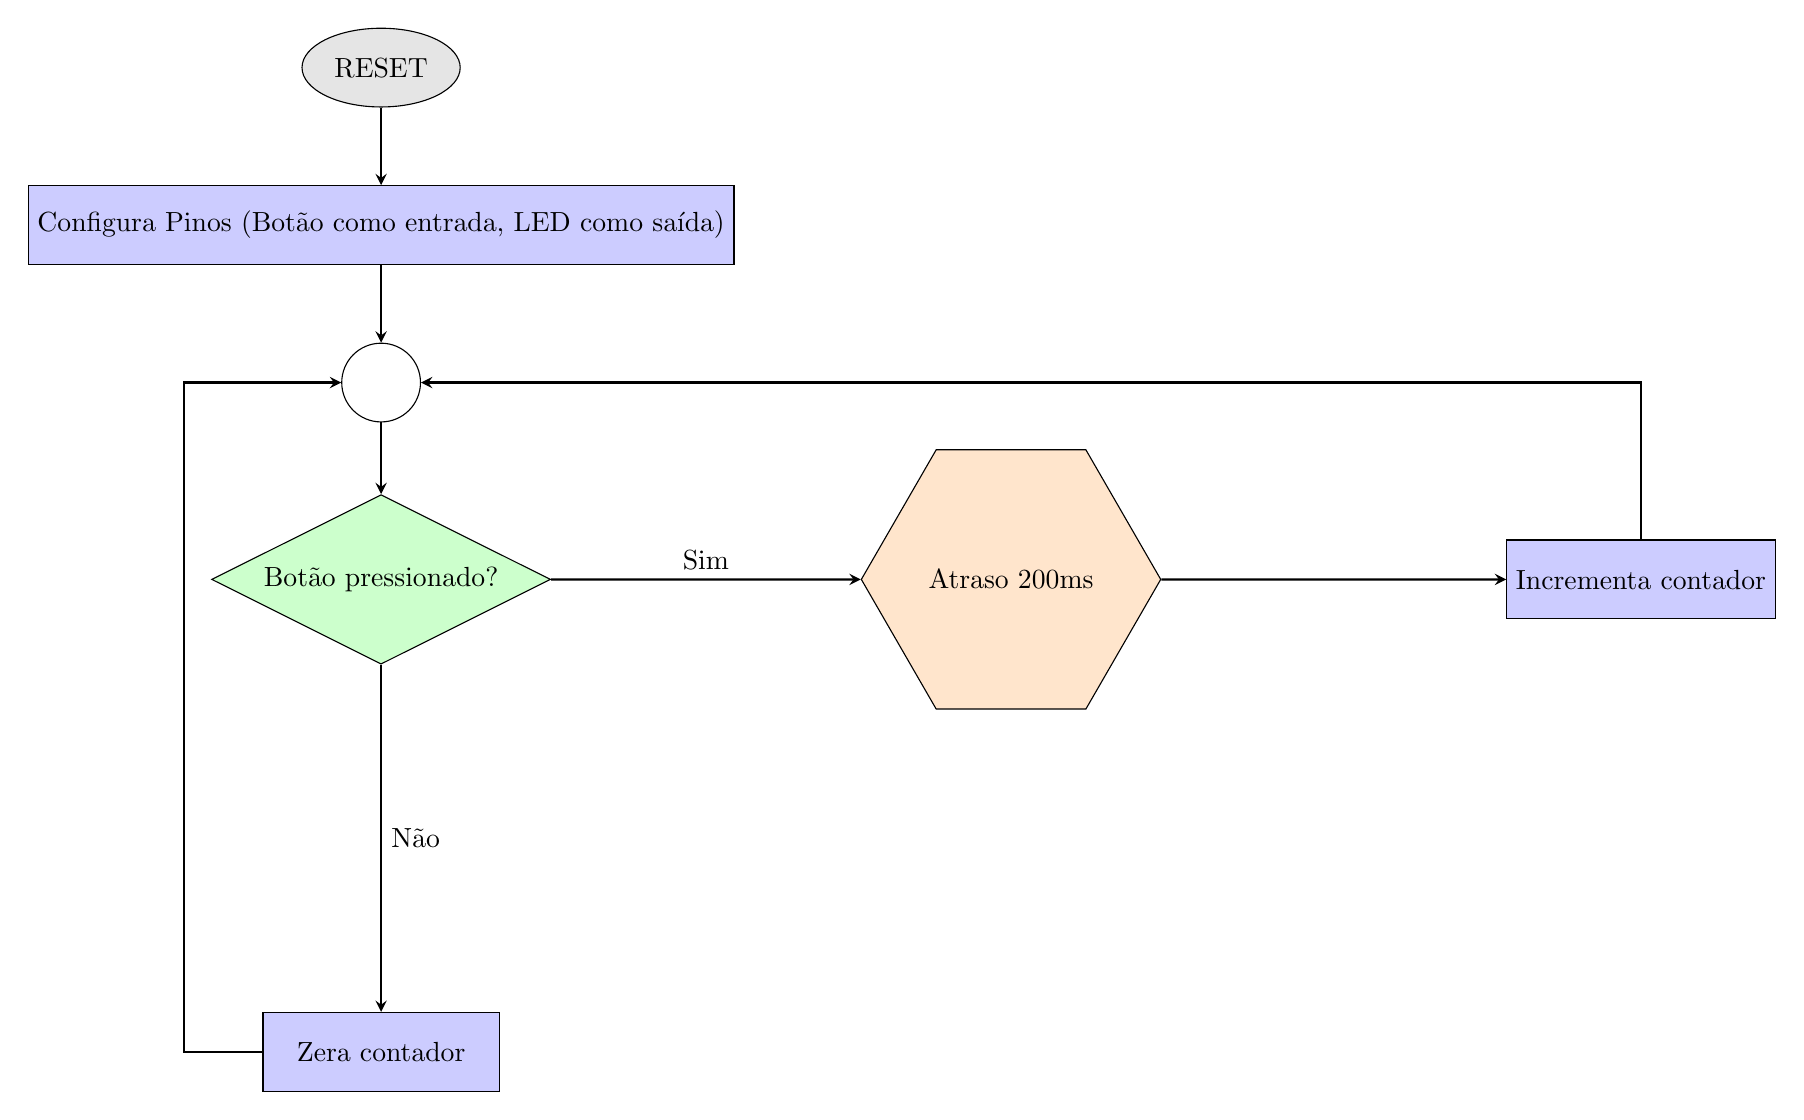
\begin{tikzpicture}[node distance=2cm]

% Nós
\node (start) [startstop] {RESET};
\node (config) [process, below of=start] {Configura Pinos (Botão como entrada, LED como saída)};
\node (circle) [bola,below of=config]{};
\node (press) [decision, below of=circle, yshift=-0.5cm] {Botão pressionado?};
\node (delay) [delay, right of=press,xshift=6cm]{Atraso 200ms};
\node (inc) [process, right of=delay, xshift=6cm] {Incrementa contador};
\node (reset) [process, below of=press, yshift=-4cm] {Zera contador};

% Conexões
\draw [arrow] (start) -- (config);
\draw [arrow] (config) -- (circle);
\draw [arrow] (circle) -- (press);

\draw [arrow] (press.east) -- (delay.west) node[midway, above] {Sim};
\draw [arrow] (delay.east) -- (inc.west);
\draw [arrow] (inc.north) |- (circle.east);

\draw [arrow] (press.south) -- (reset.north) node[midway, right] {Não};
\draw [arrow] (reset.west) -| ++(-1,0) |- (circle);



\end{tikzpicture}
\end{document}
